\section{Model}
%Model - Drawing, equations, linear equations.
The quadcopter free body diagram is shown in \autoref{droneDiagram}. 
\begin{figure}[H]
	\centering
	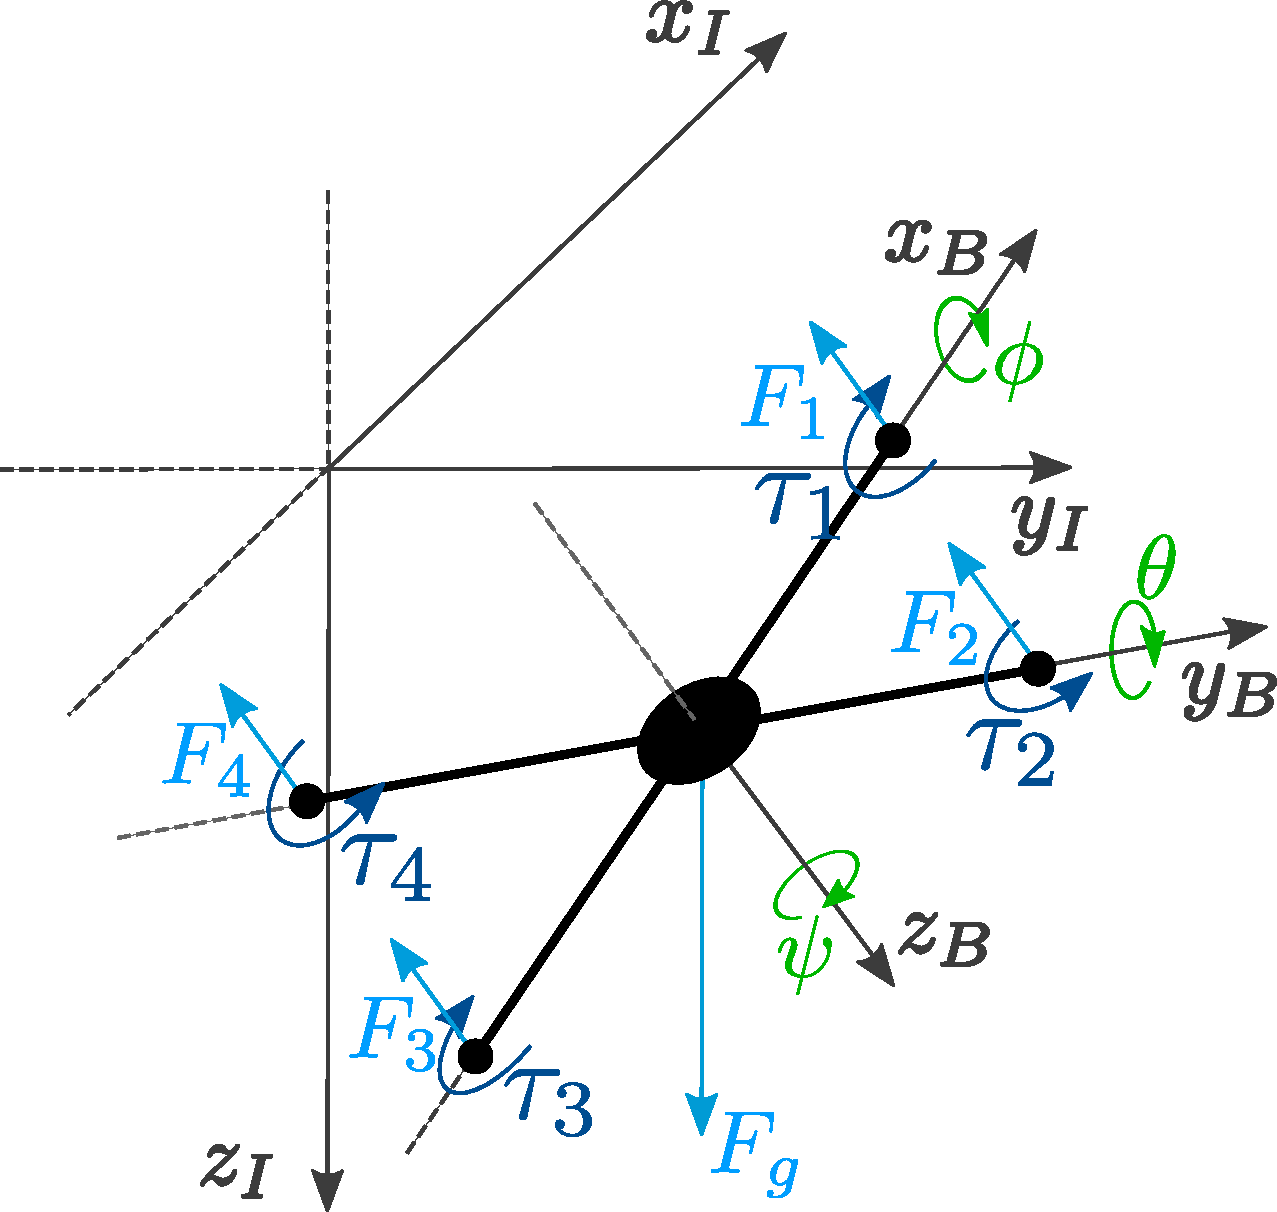
\includegraphics[scale=0.25]{figures/droneDiagram}
	\caption{Forces and torques acting on the quadcopter and the positive references chosen for rotations and translations in both inertial and body coordinate frames.}
	\label{droneDiagram}
\end{figure}
%
As it is seen, the system is modelled by using two coordinate frames. The inertial frame is utilized to describe the translational movement while the body frame is attached to the quadcopter and used to characterize its attitude behavior. In the figure, also the positive references for rotational and translational movements are depicted, as well as the main forces and torques acting on the quadcopter. 

The forces generated in the propeller are readily obtained in the body coordinate frame. In order to represent them in the inertial frame a rotation matrix is used. It is built considering a 123 rotation sequence \cite{rotationmatrix}.
 
The dynamic model of the quadcopter can be explained through three sets of equations. The first describes the motor and the propeller, the second presents the attitude response of the quadcopter and the third explains how the translational variables of the system evolve.

\subsection{Motor and Propeller}
The four motors in the quadcopter generate a rotation in the propellers that creates the force that lifts the quadcopter. The thrust force can be modeled as proportional to the square of the motor rotational speed. The thrust coefficient for one motor is found experimentally. 
 
The rotation also generates a torque on each motor due to the aerodynamic drag. Drag torque is compensated in the quadcopter by having two of the motors turning in one direction and the two others in the opposite direction. It is as well described as proportional to the square of the rotational speed in terms of a drag coefficient, which is also obtained experimentally.

The expressions for the thrust force and drag torque caused by the rotation of each propeller are
%
\begin{flalign}
	F&=k_{\mathrm{th}}\omega^2\label{eq:thrustForce}\\
	\tau&=k_{\mathrm{d}}\omega^2\label{eq:dragTorque}
\end{flalign}
%
\noindent where $F$ is the thrust force, $k_{th}$ is the thrust coefficient, $\omega$ is the angular speed of the motor, $\tau$ is the drag torque and $k_d$ is the drag coefficient.
%\begin{where}
%  \va{F}{is the thrust force}{N}
%  \va{k_{th}}{is the thrust coefficient}{N\  s^2 \  rad^{-2}}
%  \va{\omega}{is the angular velocity}{rad s^-1}
%  \va{\tau}{is the drag torque}{N m}
%  \va{k_d}{is the drag coefficient}{N \  m\  s^2 \  rad^{-2}}
%\end{where}

These equations are used in the attitude and translational models presented below.
%
\subsection{Attitude Model}
The attitude model equations, which are based on Newton's Second Law for rotational movement, are as follows 
%
\begin{flalign}
	J_x\ddot{\phi}&=k_{th} (\omega^2_4-\omega^2_2)  L \label{eq:AngleEqVelocities1}\\
	J_y \ddot{\theta}&=k_{th} (\omega^2_1-\omega^2_3)  L \label{eq:AngleEqVelocities2} \\
	J_z\ddot{\psi}&=k_d (\omega^2_1-\omega^2_2+\omega^2_3-\omega^2_4)\label{eq:AngleEqVelocities3}
\end{flalign}

\noindent where $J_x$, $J_y$ and $J_z$ are the moments of inertia around the three axes of rotation, $\ddot{\phi}$, $\ddot{\theta}$ and $\ddot{\psi}$ are the accelerations in roll, pitch and yaw angles, respectively, $\omega_i$ is the rotational speed of each motor and $L$ is the distance between the center of the quadcopter and the position of the motors.

The expressions above state how the thrust forces and the drag torques generated on the propellers affect the attitude behavior of the quadcopter.  
\subsection{Translational Model}
The equations describing the response of the system along the inertial x, y and z axes are derived from Newton's Second Law. The forces that act on the system are those from the propellers and the gravitational force. These expressions are
%
\begin{flalign}
     m\ddot{x}_I = &-k_{th} ({\omega_1}^2+{\omega_2}^2+{\omega_3}^2+{\omega_4}^2) \\
     & \mathrm{x} (\cos\phi \sin\theta \cos\psi + \sin\phi\sin\psi)   \label{eq:AccelerationEqInertial1}\nonumber\\
     m \ddot{y}_I = &-k_{th}({\omega_1}^2+{\omega_2}^2+{\omega_3}^2+{\omega_4}^2)\\
     & \cdot (\cos(\phi) \sin\theta \sin(\psi) - \sin(\phi)\ \cos(\psi))  \label{eq:AccelerationEqInertial2}\nonumber\\
     m\ \ddot{z}_I = &F_g-k_{th}\ ({\omega_1}^2+{\omega_2}^2+{\omega_3}^2+{\omega_4}^2)\\
     & \cdot \cos(\phi)\ \cos(\theta)
     \label{eq:AccelerationEqInertial3}\nonumber
\end{flalign}
\noindent where $m$ is the mass of the quadcopter, $\ddot{x}_I$, $\ddot{y}_I$ and $\ddot{z}_I$ are the accelerations along the inertial reference frame directions, $\phi$, $\theta$ and $\psi$ are the roll, pitch and yaw angles respectively and $F_g$ is the gravitational force acting on the quadcopter.

It is worth mentioning that, as the thrust forces always point in the negative ${z}_B$ direction, the accelerations along ${x}_I$ and ${y}_I$ directions are zero when pitch and roll angles are zero.

\subsection{Linearization}
The model equations are linearized using the first order Taylor approximation around an equilibrium point of the system. The chosen point is the hovering position, which implies that all variables have a value of zero, that is, the attitude and translational accelerations, velocities and positions. Choosing a zero acceleration equilibrium point along the ${z}_I$ axis yields an equilibrium rotational speed so that the necessary thrust is generated to compensate for the gravitational force. The relation is expressed as
\begin{flalign}
    \overline{\omega}_i=\sqrt{\frac{m\  g}{4k_{th}}}
    \label{eq:equilibriumomegas}
\end{flalign}
The resulting equations for the attitude model after the linearization are shown in \autoref{eqAngleLin1}, \ref{eqAngleLin2} and \ref{eqAngleLin3}. 
\begin{flalign}
  J_x\ \Delta\ddot{\phi}   = \ &2\ k_{th}\ L\ {\overline{\omega}_4}\ \Delta \omega_4\ -\ 2\ k_{th}\ L\ {\overline{\omega}_2}\ \Delta \omega_2
  \label{eqAngleLin1} \\
  J_y\ \Delta\ddot{\theta} = \ &2\ k_{th}\ L\ \overline{\omega}_1\ \Delta \omega_1\ -\ 2\ k_{th}\ L\ \overline{\omega}_3\ \Delta \omega_3
  \label{eqAngleLin2} \\
  J_z\ \Delta\ddot{\psi}   = \ &2\ k_d\ {\overline{\omega}_1}\ \Delta \omega_1\ -\ 2\ k_d\ {\overline{\omega}_2}\ \Delta \omega_2\ \label{eqAngleLin3}
  \\ & +\ 2\ k_d\ {\overline{\omega}_3}\ \Delta \omega_3\ -\ 2\ k_d\ {\overline{\omega}_4}\ \Delta \omega_4\nonumber  
\end{flalign}
\noindent where $\Delta\ddot{\phi}$, $\Delta\ddot{\theta}$ and $\Delta\ddot{\psi}$ are the changes in rotational acceleration from equilibrium, $\overline{\omega}_i$ is the rotational speed of each motor in equilibrium and $\Delta \omega_i$ is the change in rotational speed of each motor from equilibrium. 

Similarly, the equations of the translational model are linearized. The result is
\begin{flalign}
  m\ \Delta\ddot{x}_I =\ &-k_{th}\ ({\overline{\omega}_1}^2+{\overline{\omega}_2}^2+{\overline{\omega}_3}^2+{\overline{\omega}_4}^2)\  \Delta\theta \label{eq:TransLinearEquations1} \\
  m\ \Delta\ddot{y}_I =\ & k_{th}\ ({\overline{\omega}_1}^2+{\overline{\omega}_2}^2+{\overline{\omega}_3}^2+{\overline{\omega}_4}^2)\ \Delta\phi \label{eq:TransLinearEquations2}\\
  m\ \Delta\ddot{z}_I =\ &-2\ k_{th}\ \overline{\omega}_1\ \Delta\omega_1 -2\ k_{th}\ \overline{\omega}_2\ \Delta\omega_2 \label{eq:TransLinearEquations3} \\
  &\ \ -2\ k_{th}\ \overline{\omega}_3\ \Delta\omega_3-2\ k_{th}\ \overline{\omega}_4\ \Delta\omega_4\ \nonumber 
\end{flalign} 
\noindent where $\Delta\ddot{x_I}$, $\Delta\ddot{y_I}$ and $\Delta\ddot{z_I}$ are the changes in linear acceleration from equilibrium in each direction of the inertial frame and $\Delta \phi$ and $\Delta \theta$ are the changes in roll and pitch from equilibrium respectively.